\documentclass[a4paper, 12pt]{article}

% Language setting
% Replace `english' with e.g. `spanish' to change the document language
\usepackage[portuguese]{babel}

% Set page size and margins
% Replace `letterpaper' with `a4paper' for UK/EU standard size
\usepackage[letterpaper,top=2cm,bottom=2cm,left=3cm,right=3cm,marginparwidth=1.75cm]{geometry}
\usepackage[utf8]{inputenc}
\usepackage{listings}
\usepackage{amsmath, amsfonts, amssymb}


% Useful packages
\usepackage{amsmath}
\usepackage{esint}
\usepackage{setspace}
\usepackage{graphicx}
\usepackage[colorlinks=true, allcolors=blue]{hyperref}


\title{Desafio De Matemática}
\author{Mario Ambrosio De Souza Neto}
\date{}

\onehalfspace
\begin{document}
\maketitle

\section{- Deduza a o determinante 4x4 usado a formula. $$det(A) =\sum_{\sigma\in sn} (\prod_{i=1}^{n} (-1)^{sgn(\sigma)} a_{i\sigma}(i))$$}


\textbf{Resultado:}

$$det(A) =\sum_{\sigma\in s_4} (\prod_{i=1}^{4} (-1)^{sgn(\sigma)} a_{i\sigma}(i))=\prod_{i=1}^{4} (-1)^{sgn(1234)} a_{i1234}(i) + \prod_{i=1}^{4} (-1)^{sgn(1243)} a_{i1243}(i) + $$

$$\prod_{i=1}^{4} (-1)^{sgn(1324)} a_{i1324}(i) + \prod_{i=1}^{4} (-1)^{sgn(1342)} a_{i1342}(i) + \prod_{i=1}^{4} (-1)^{sgn(1423)} a_{i1423}(i) + \prod_{i=1}^{4} (-1)^{sgn(1432)} a_{i1432}(i) +$$

$$\prod_{i=1}^{4} (-1)^{sgn(2134)} a_{i2134}(i) + \prod_{i=1}^{4} (-1)^{sgn(2143)} a_{i2143}(i) + \prod_{i=1}^{4} (-1)^{sgn(2314)} a_{i2314}(i) + \prod_{i=1}^{4} (-1)^{sgn(2341)} a_{i2341}(i) +$$

$$\prod_{i=1}^{4} (-1)^{sgn(2413)} a_{i2413}(i) + \prod_{i=1}^{4} (-1)^{sgn(2431)} a_{i2431}(i) + \prod_{i=1}^{4} (-1)^{sgn(3124)} a_{i3124}(i) + \prod_{i=1}^{4} (-1)^{sgn(3142)} a_{i3142}(i) +$$

$$\prod_{i=1}^{4} (-1)^{sgn(3214)} a_{i3214}(i) + \prod_{i=1}^{4} (-1)^{sgn(3241)} a_{i3241}(i) + \prod_{i=1}^{4} (-1)^{sgn(3412)} a_{i3412}(i) + \prod_{i=1}^{4} (-1)^{sgn(3421)} a_{i3421}(i) +$$

$$\prod_{i=1}^{4} (-1)^{sgn(4123)} a_{i4123}(i) + \prod_{i=1}^{4} (-1)^{sgn(4132)} a_{i4132}(i) + \prod_{i=1}^{4} (-1)^{sgn(4213)} a_{i4213}(i) + \prod_{i=1}^{4} (-1)^{sgn(4231)} a_{i4231}(i) +$$

$$\prod_{i=1}^{4} (-1)^{sgn(4312)} a_{i4312}(i) + \prod_{i=1}^{4} (-1)^{sgn(4321)} a_{i4321}(i)$$

=\leftline{ ($a^{11}$ · $a^{22}$ · $a^{33}$ · $a^{44}$) - ($a^{11}$ · $a^{22}$ · $a^{34}$ · $a^{43}$) - ($a^{11}$ · $a^{23}$ · $a^{32}$ · $a^{43}$) + ($a^{11}$ · $a^{23}$ · $a^{34}$ · $a^{42}$) +} 
\leftline{ ($a^{11}$ · $a^{24}$ · $a^{32}$ · $a^{43}$) - ($a^{11}$ · $a^{24}$ · $a^{33}$ · $a^{42}$) - ($a^{12}$ · $a^{21}$ · $a^{33}$ · $a^{44}$) + ($a^{12}$ · $a^{21}$ · $a^{34}$ · $a^{43}$) +} 
\leftline{ ($a^{12}$ · $a^{23}$ · $a^{31}$ · $a^{44}$) - ($a^{12}$ · $a^{23}$ · $a^{34}$ · $a^{41}$) - ($a^{12}$ · $a^{24}$ · $a^{33}$ · $a^{44}$) + ($a^{12}$ · $a^{24}$ · $a^{33}$ · $a^{41}$) +} 
\leftline{ ($a^{13}$ · $a^{21}$ · $a^{32}$ · $a^{44}$) - ($a^{13}$ · $a^{21}$ · $a^{34}$ · $a^{42}$) - ($a^{13}$ · $a^{22}$ · $a^{31}$ · $a^{44}$) + ($a^{13}$ · $a^{22}$ · $a^{34}$ · $a^{41}$) +} 
\leftline{ ($a^{13}$ · $a^{24}$ · $a^{31}$ · $a^{42}$) - ($a^{13}$ · $a^{24}$ · $a^{32}$ · $a^{41}$) - ($a^{14}$ · $a^{21}$ · $a^{32}$ · $a^{43}$) + ($a^{14}$ · $a^{21}$ · $a^{33}$ · $a^{42}$) +}
\leftline{ ($a^{14}$ · $a^{22}$ · $a^{31}$ · $a^{43}$) - ($a^{14}$ · $a^{22}$ · $a^{33}$ · $a^{41}$) - ($a^{14}$ · $a^{23}$ · $a^{31}$ · $a^{42}$) + ($a^{14}$ · $a^{23}$ · $a^{32}$ · $a^{41}$)}

\section{- Calcule o determinante, usando o que foi deduzido, de duas matrizes definidas pelo autor.}

\subsection{Matriz de det(A) = 0}
$$\left[
\begin{array}{c c c c}
0&0&1&2\\
0&1&2&3\\
1&2&3&4\\ 2&3&4&5
\end{array}\right]
$$
\textbf{Resultado:}

\centerline{det(A) = (0 · 1 · 3 · 5) - (0 · 1 · 4 · 4) - (0 · 2 · 2 · 5) + (0 · 2 · 4 · 3) +}
\centerline{(0 · 3 · 2 · 4) - (0 · 3 · 3 · 3) - (0 · 0 · 3 · 5) + (0 · 0 · 4 · 4) +}
\centerline{(0 · 2 · 1 · 5) - (0 · 2 · 4 · 2) - (0 · 3 · 1 · 4) + (0 · 3 · 3 · 2) +}
\centerline{(1 · 0 · 2 · 5) - (1 · 0 · 4 · 3) - (1 · 1 · 1 · 5) + (1 · 1 · 4 · 2) +}
\centerline{(1 · 3 · 1 · 3) - (1 · 3 · 2 · 2) - (2 · 0 · 2 · 4) + (2 · 1 · 3 · 3) +}
\centerline{(2 · 1 · 1 · 4) - (2 · 1 · 3 · 2) - (2 · 2 · 1 · 3) + (2 · 2 · 2 · 2)}\vspace{1cm}

\centerline{det(A) = 0}


\subsection{Matriz de det(A) $\neq$ 0}
$$\left[
\begin{array}{c c c c}
1&3&2&0\\
3&1&0&2\\
2&3&0&1\\ 0&2&1&3
\end{array}\right]
$$
\textbf{Resultado:}

\centerline{det(A) = (1 · 1 · 0 · 3) - (1 · 1 · 1 · 1) - (1 · 0 · 3 · 3) + (1 · 0 · 1 · 2) +}
\centerline{(1 · 2 · 3 · 1) - (1 · 2 · 0 · 2) - (3 · 3 · 0 · 3) + (3 · 3 · 1 · 1) +}
\centerline{(3 · 0 · 2 · 3) - (3 · 0 · 1 · 0) - (3 · 2 · 2 · 1) + (3 · 2 · 0 · 0) +}
\centerline{(2 · 3 · 3 · 3) - (2 · 3 · 1 · 2) - (2 · 1 · 2 · 3) + (2 · 1 · 1 · 0) +}
\centerline{(2 · 2 · 2 · 2) - (2 · 2 · 3 · 0) - (0 · 3 · 3 · 1) + (0 · 3 · 0 · 2) +}
\centerline{(0 · 1 · 2 · 1) - (0 · 1 · 0 · 0) - (0 · 0 · 2 · 2) + (0 · 0 · 3 · 0)}\vspace{1cm}

\centerline{det(A) = 48}

\section{- Programar o metodo em python. Verifique os resultados, mostre o console.}

\begin{scriptsize}
\subsection{Código}
\begin{lstlisting}
def pegarMenor(matrix, i, j):
    return [row[:j] + row[j+1:] for row in (matrix[:i] + matrix[i+1:])]

def determinante(matrix):
    if len(matrix) == 2:
        return matrix[0][0] * matrix[1][1] - matrix[0][1] * matrix[1][0]
    else:
        det = 0
        for i in range(len(matrix)): 
            menor = pegarMenor(matrix, 0, i)
            cofactor = (-1) ** (i % 2) * determinante(menor)
            det += matrix[0][i] * cofactor
        return det

A = [[0, 0, 1, 2], [0, 1, 2, 3], [1, 2, 3, 4], [2, 3, 4, 5]] # Codigo do exemplo 2.1
B = [[1, 3, 2, 0], [3, 1, 0, 2], [2, 3, 0, 1], [0, 2, 1, 3]] # Codigo do exemplo 2.2
detA = determinante(A)
detB = determinante(B)

print(f"Resultado da Matriz de det(A) == 0 : {detA}")
print(f"Resultado da Matriz de det(A) != 0 : {detB}")
\end{lstlisting}
\end{scriptsize}

\subsection{Resultado no console}
\center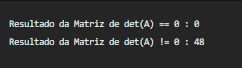
\includegraphics{Console.jpg}

\end{document}